\chapter{User Authentication/Authorization}
\label{appendix:design:alternatives:auth}

User Authentication/Authorization is an important aspect of the solution. During the requirements elicitation, mentioned in Section~\ref{subsec:requirements:functional:roles}, it was clear that several different levels of permissions had to be given to Tenants. These levels of permissions also had to be managed by someone. As such, users had to be authenticated in the system and all accesses had to be authorized.

Four approaches were considered:

\begin{itemize}
   \item \nameref{subsubsec:design:alternatives:auth:internalauth};
   \item \nameref{subsubsec:design:alternatives:auth:externalauth};
   \item \nameref{subsubsec:design:alternatives:auth:externalauthinternalpermission};
   \item \nameref{subsubsec:design:alternatives:auth:externalauthinternaloauth}.
\end{itemize}

The fourth option was the approach taken.

\section{Internal Authentication Server}
\label{subsubsec:design:alternatives:auth:internalauth}

By creating an Internal Authentication Server we could have a normal, private and controlled user authentication/authorization flow in the environment. Both user credentials and permissions would be managed internally.

The following diagram, Figure~\ref{fig:design:alternatives:auth:internalauth:diagram},presents the normal environment flow for this alternative.

\begin{figure}[H]
   \centering
   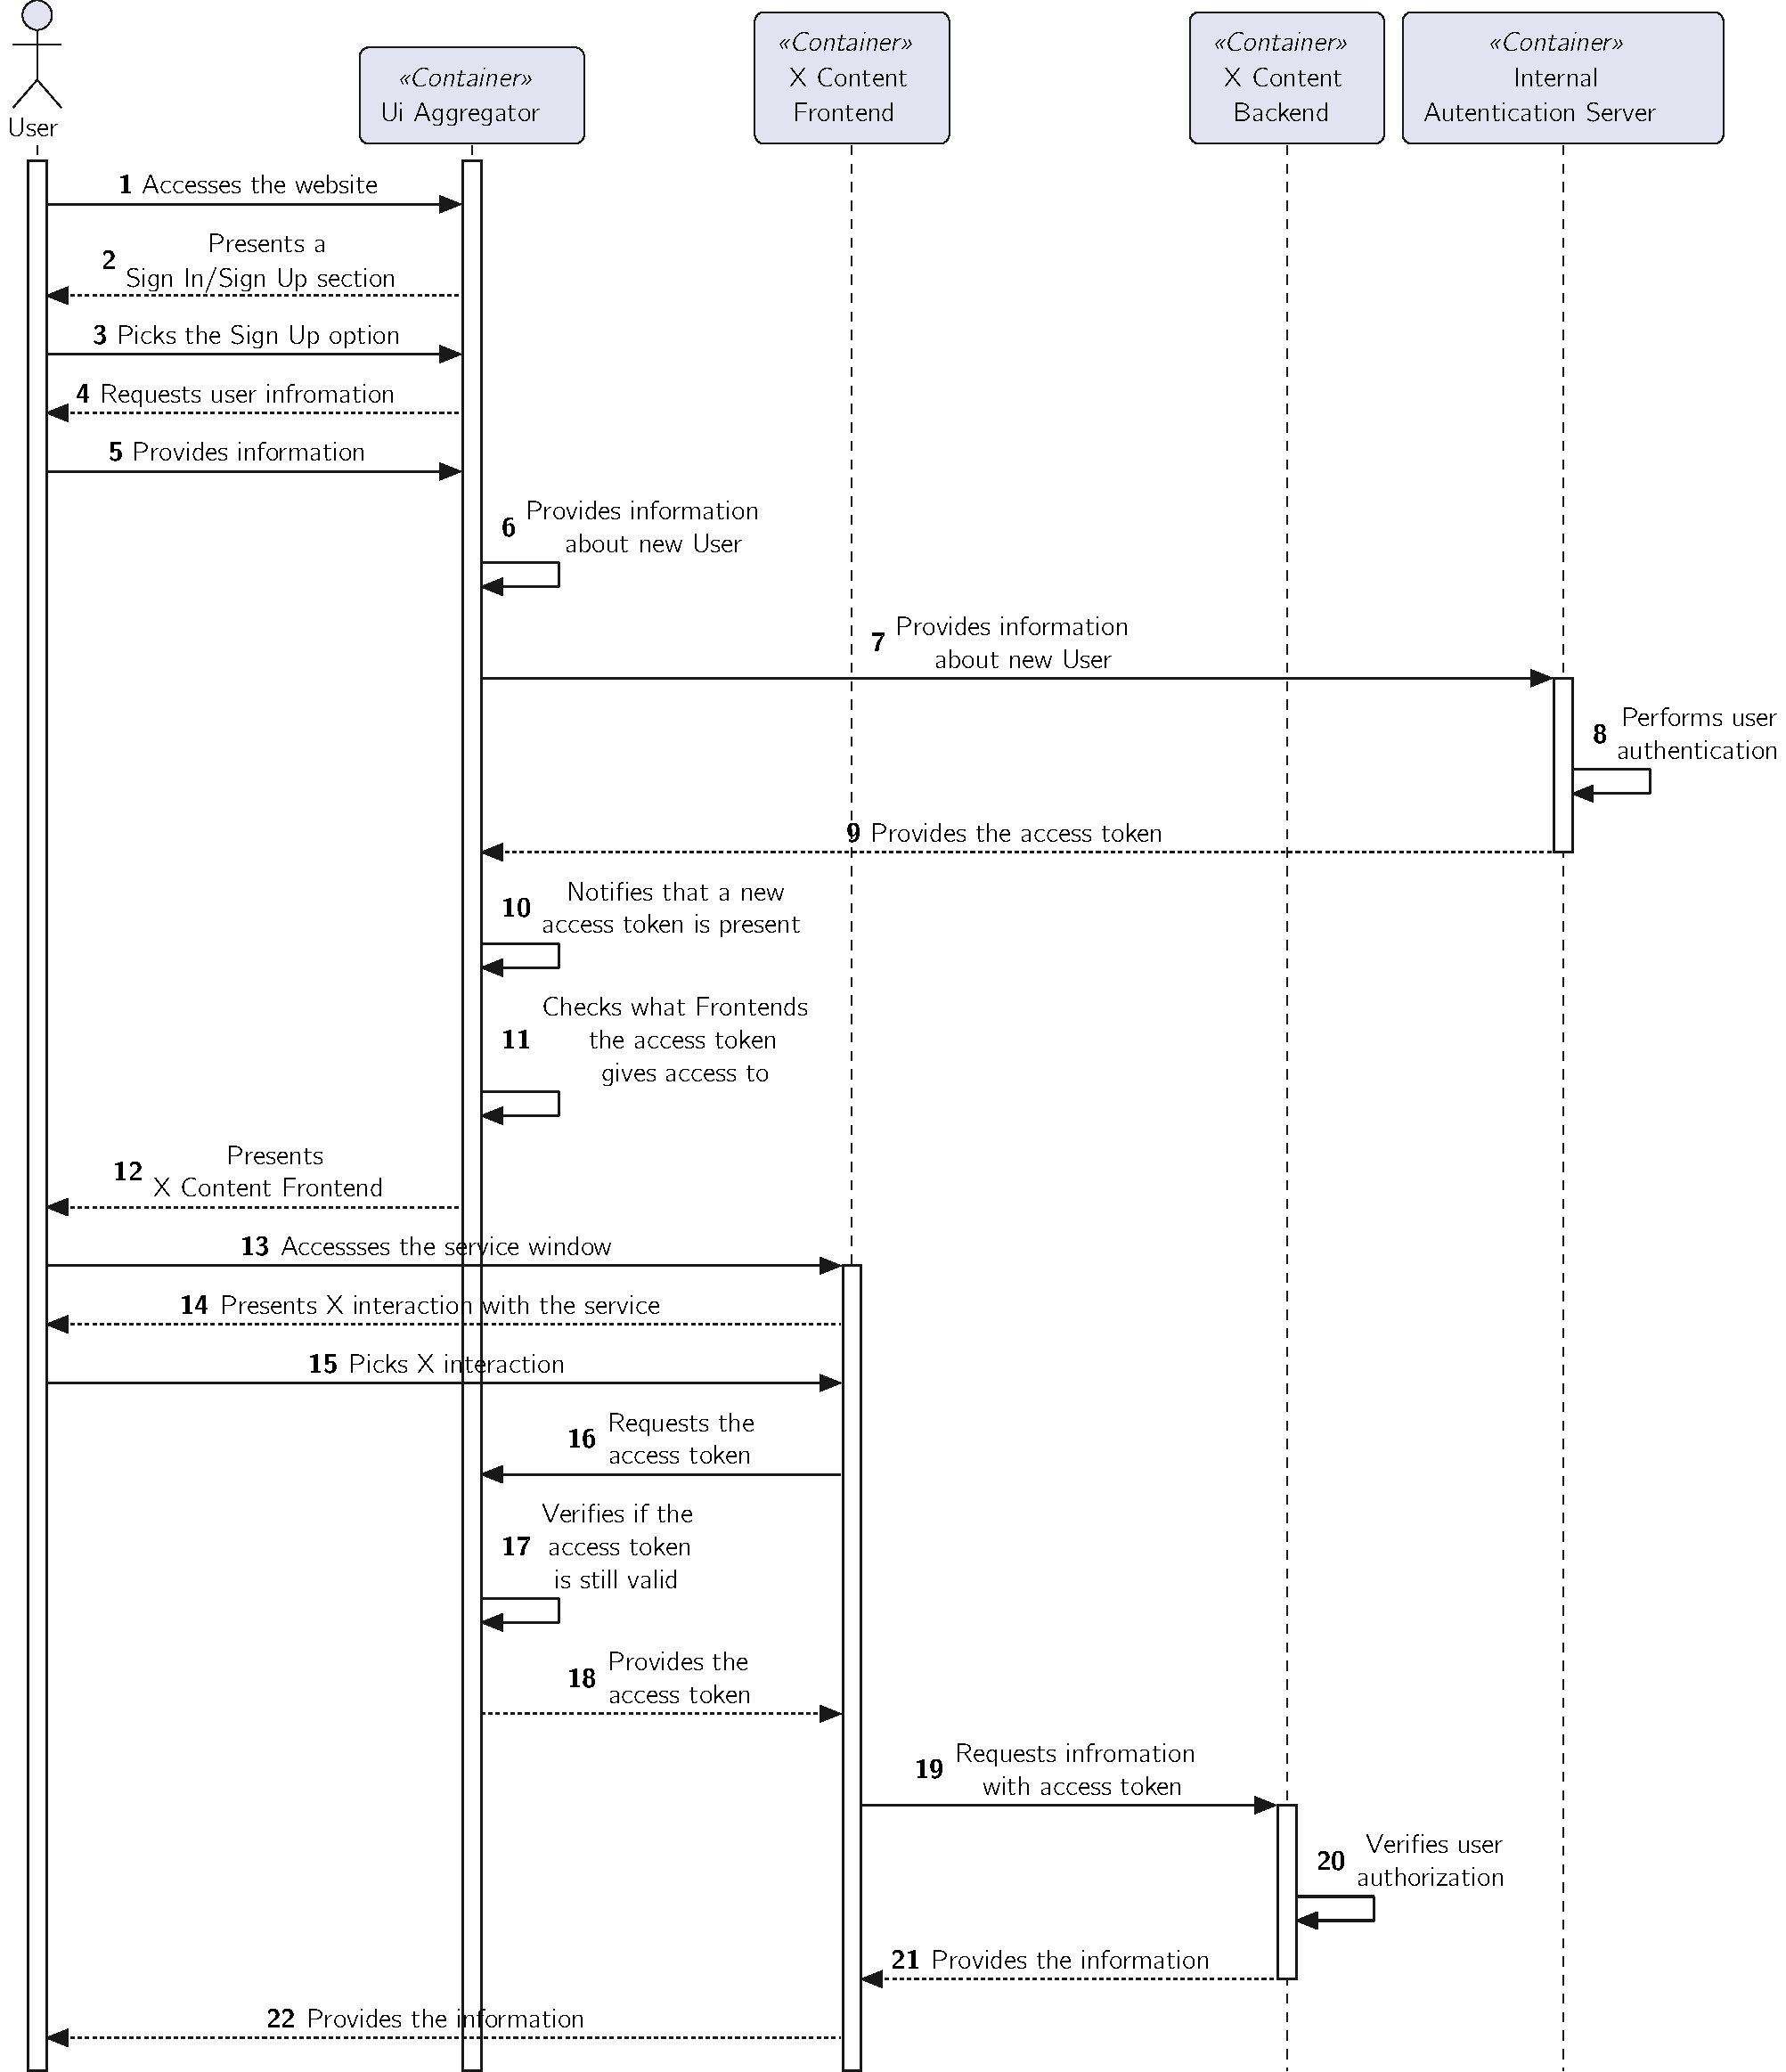
\includegraphics[page=1,width=\columnwidth]{assets/diagrams/design/alternatives/auth/alternative1.pdf}
   \caption[User Authentication/Authorization - Internal Authentication Server Alternative - Sequence Diagram]{User Authentication/Authorization - Internal Authentication Server Alternative - Sequence Diagram}
   \label{fig:design:alternatives:auth:internalauth:diagram}
\end{figure}

This alternative introduces the need to internally secure user credentials and other sensitive information from data breaches. It would also require each user to register in sensae with a new account credentials. For this reasons this alternative was discarded.

\section{External Authentication Server}
\label{subsubsec:design:alternatives:auth:externalauth}

By using an External Authentication Server there would be no need to store user credentials or permissions. This services are commonly identified as \gls{CIAM} solutions. According to \cite{ciam} these solutions include features such as ``self-service for registration, password and consent management, profile generation and management, authentication and authorization into applications, identity repositories, reporting and analytics, APIs and SDKs for mobile applications, and social identity registration and login''.

The following diagram, Figure~\ref{fig:design:alternatives:auth:externalauth:diagram}, presents the normal environment flow for this alternative.

\begin{figure}[H]
   \centering
   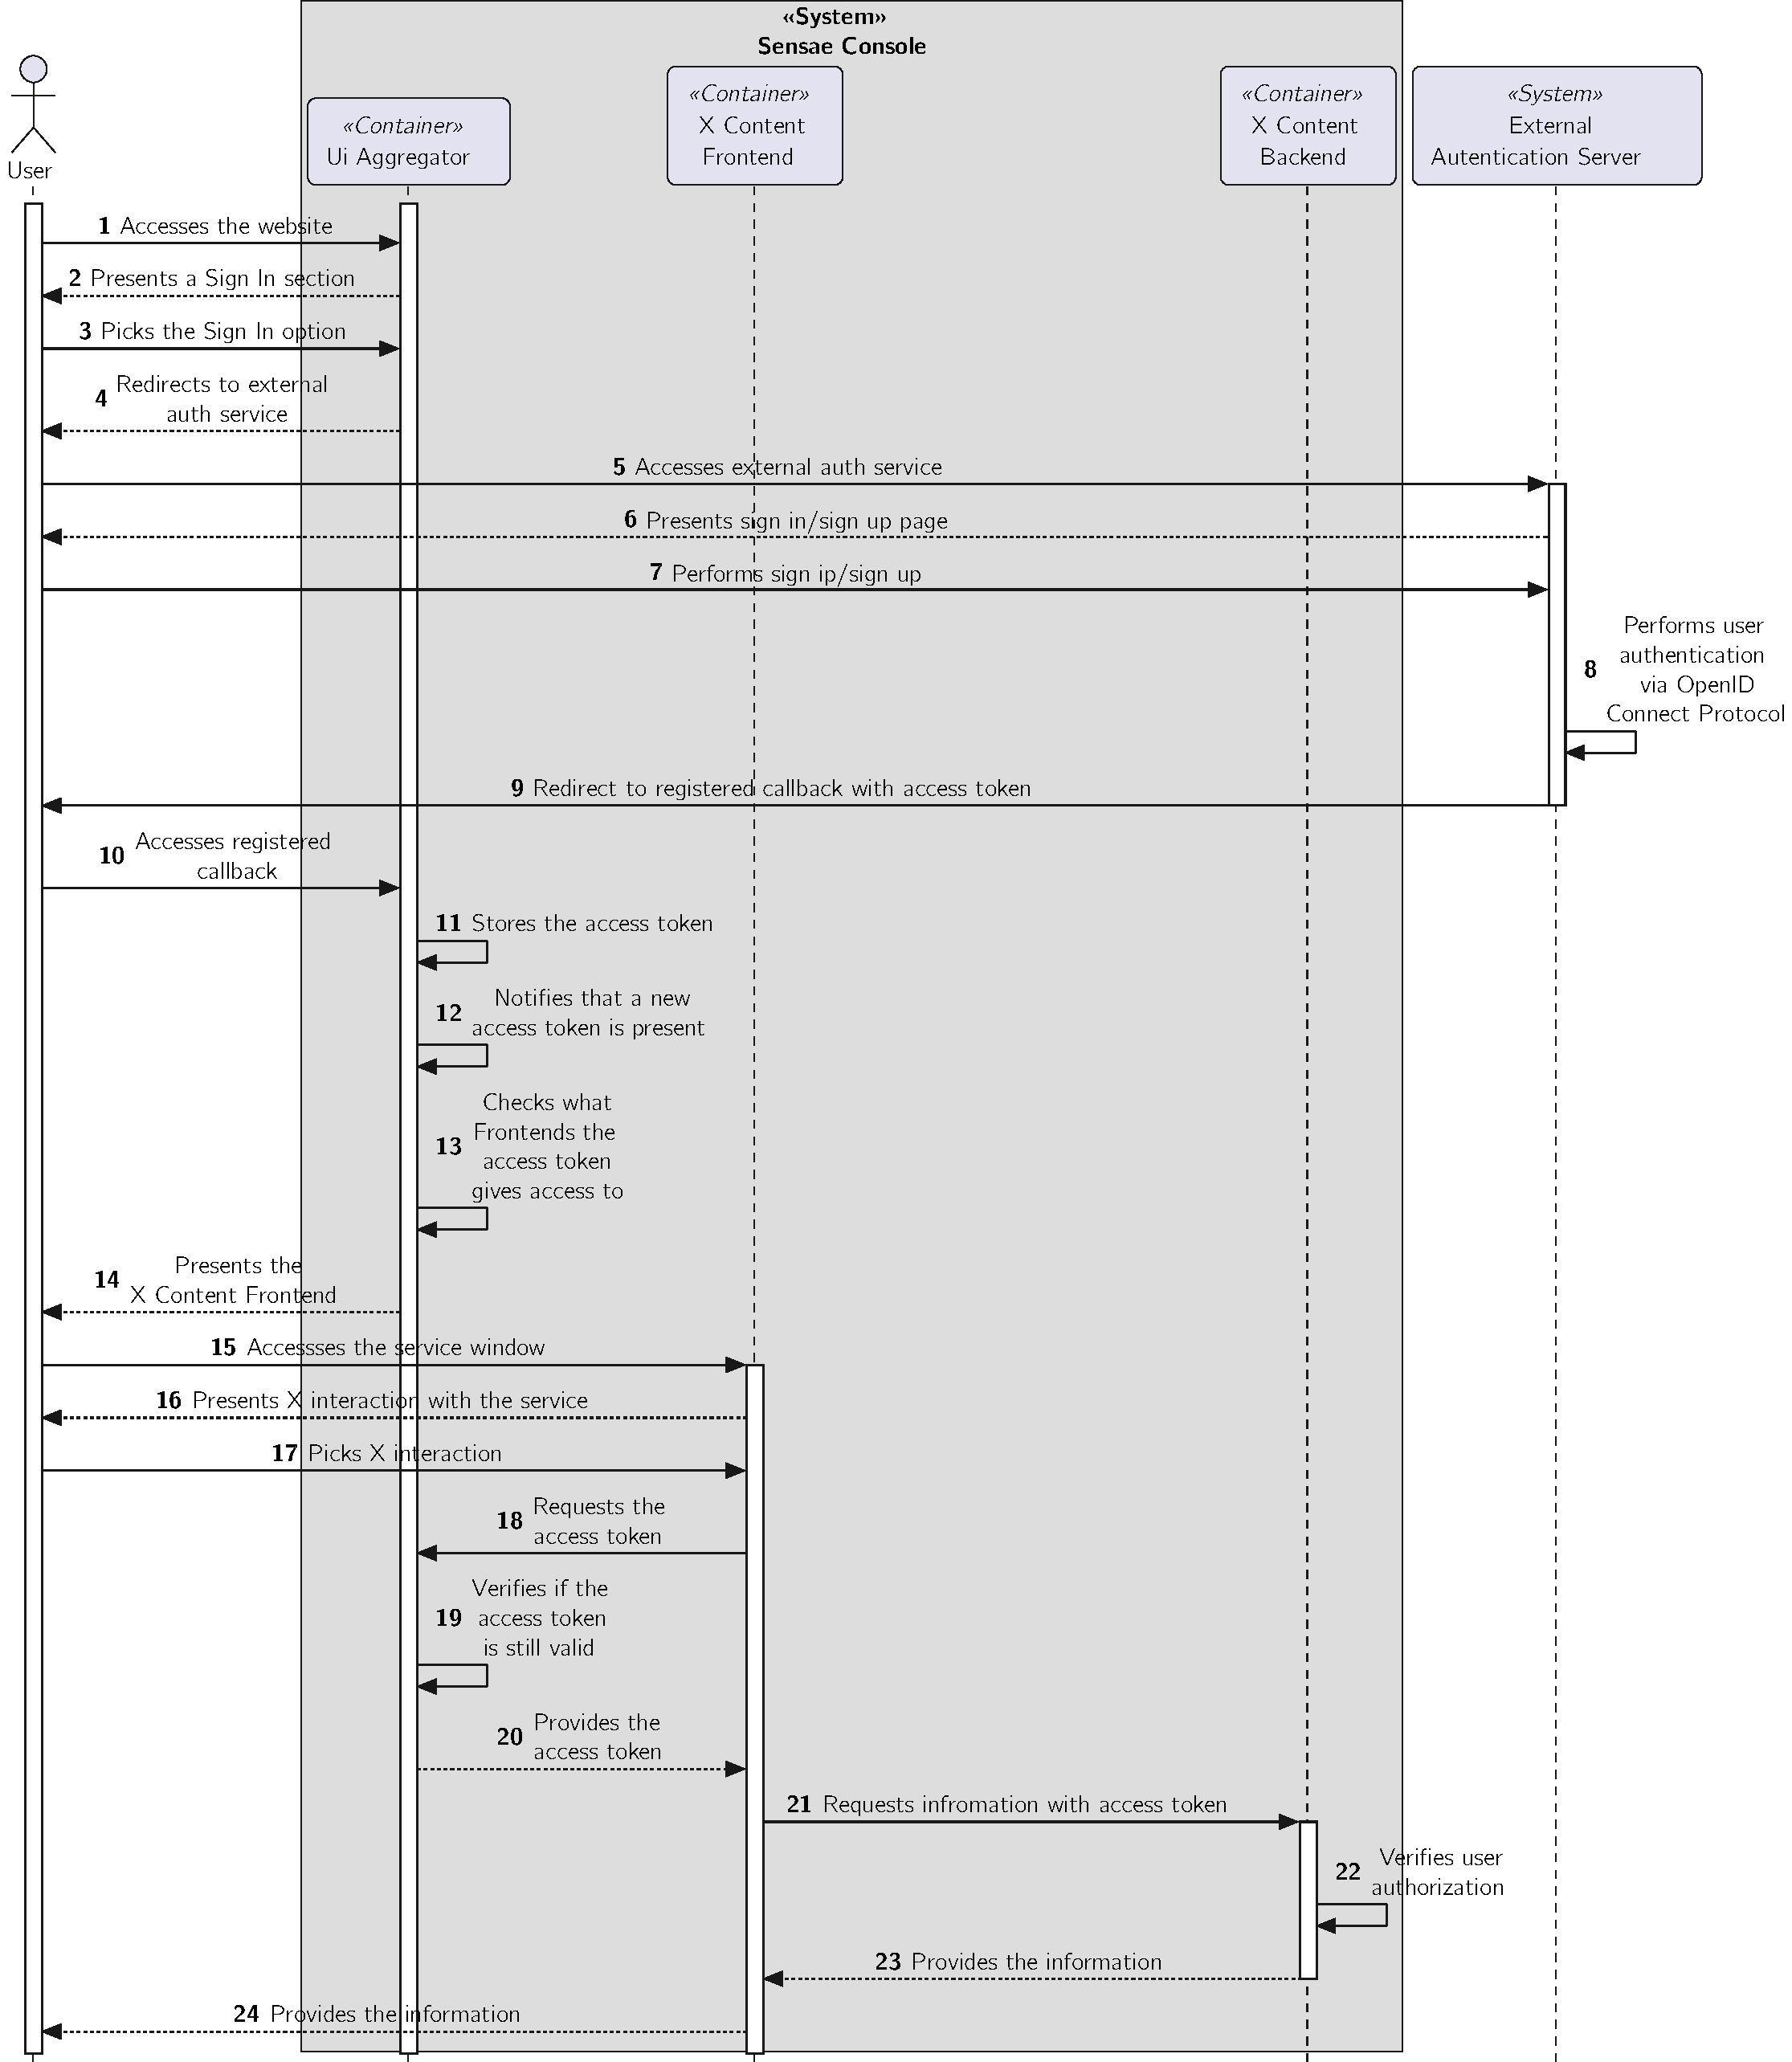
\includegraphics[page=1,width=\columnwidth]{assets/diagrams/design/alternatives/auth/alternative2.pdf}
   \caption[User Authentication/Authorization - External Authorization Server Alternative - Sequence Diagram]{User Authentication/Authorization - External Authorization Server Alternative - Sequence Diagram}
   \label{fig:design:alternatives:auth:externalauth:diagram}
\end{figure}

This approach would create a strong dependency to the \gls{CIAM} solution used since all user credentials and authorization level would have to be managed by the \gls{CIAM} solution.
Some of this services are: (i) \citetitle{auth0id}, (ii) \citetitle{googleid}, (iii) \citetitle{oktaid}, (iv) \citetitle{amazonid} and (v) \citetitle{azureid}.

The platform Auth0 was tested and is capable of answering all of this project's requirements.

As stated before, the dependency created would force the environment to always be coupled to the chosen \gls{CIAM} solution. For this reason this alternative was discarded.

\section{External Authentication Server with Internal Authorization Server}
\label{subsubsec:design:alternatives:auth:externalauthinternalpermission}

By using an External Authentication Server there would be no need to store user credentials, the user authorization aspects would then be managed internally via and \textit{Authorization Server}.

The following diagram, Figure~\ref{fig:design:alternatives:auth:externalauthinternalpermission:diagram}, presents the normal environment flow for this alternative.

\begin{figure}[H]
   \centering
   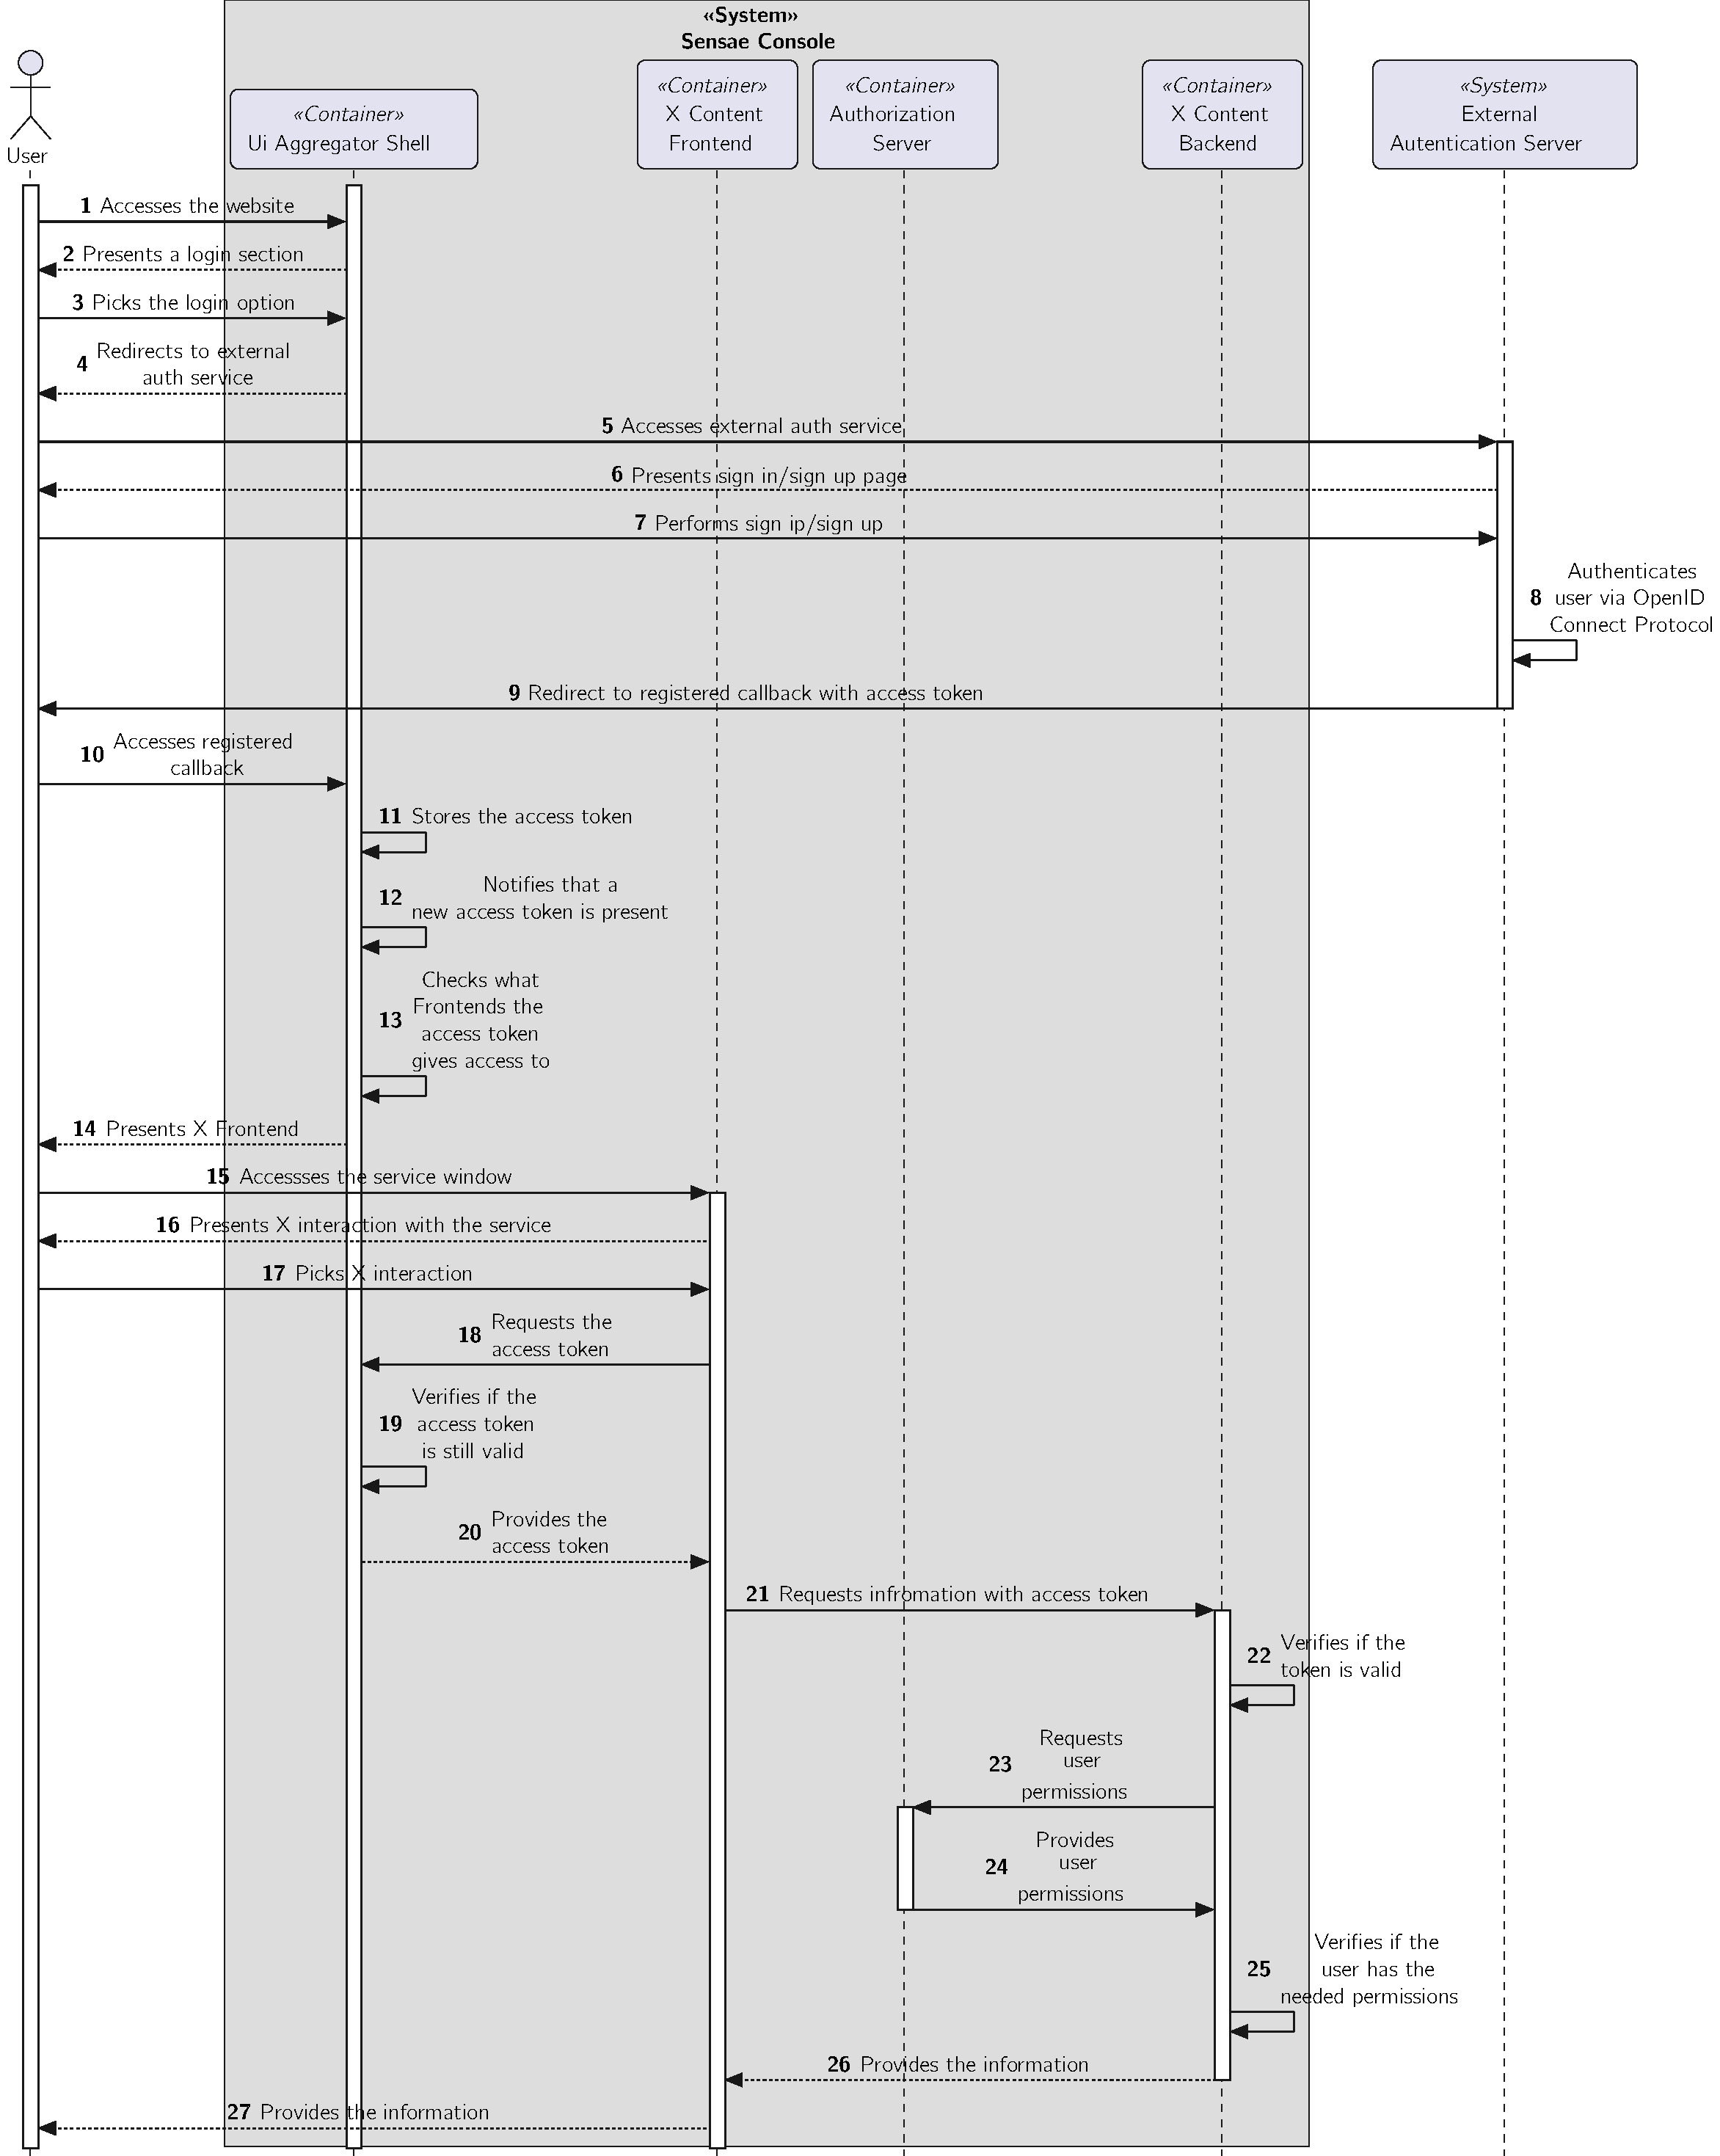
\includegraphics[page=1,width=\columnwidth]{assets/diagrams/design/alternatives/auth/alternative3.pdf}
   \caption[User Authentication/Authorization - External Authentication Server with Internal Authorization Server Alternative - Sequence Diagram]{User Authentication/Authorization - External Authentication Server with Internal Authorization Server Alternative - Sequence Diagram}
   \label{fig:design:alternatives:auth:externalauthinternalpermission:diagram}
\end{figure}

This approach would create a dependency to the \gls{CIAM} solution used and presented in the second alternative.

This dependency is less severe compared with the second alternative since all authorization aspects would be managed internally.
This approach would require any backend to query the \textit{Authorization Server} for user permissions so that it could verify if the user was authorized to preform the requested action or not. This would therefore linger down the performance of the system since each action would have to be verified in a single container: the \textit{Authorization Server}.

\section{External Authentication Server with Internal Oauth2 Server}
\label{subsubsec:design:alternatives:auth:externalauthinternaloauth}

By using an external Authorization Server there would be no need to store user credentials. An internal Oauth2 Server would remove the direct dependency to the \textit{Permissions Server} presented in the third alternative.

This alternative is introduced in Figure~\ref{fig:design:architecture:platform:container:process:diagram:authentication} and Figure~\ref{fig:design:architecture:platform:container:process:diagram:authorization} where the Internal Oauth2 Server is the Identity Management Backend.

This approach would create a dependency to the \gls{CIAM} solution used and presented in the second alternative. This dependency is less severe compared with the second alternative since all user permissions would be managed internally.
This approach would require the system to create and refresh \textit{access tokens} based on the \textit{id token} received by the external \gls{CIAM} solution. Contrary to the third alternative it would not create excessive pressure in a specific container.

This approach also allows the system to easily integrate with more than one \gls{CIAM} solution while managing user permissions in a single place. The \gls{CIAM} solutions that \textbf{Sensae Console} is integrated with are:

\begin{itemize}
   \item Google Identity Platform: for common individuals that want to use the system, since almost everyone has a google account;
   \item Azure Active Directory: for companies and organizations since most use Office 365 services internally.
\end{itemize}

Due to the reasons presented above, this was the adopted approach.
